%%%%%%%%%%%%%%%%%%%%%%%%%%%%%%%%%%%%%%%%%
% baposter Portrait Poster
% LaTeX Template
% Version 1.0 (15/5/13)
%
% Created by:
% Brian Amberg (baposter@brian-amberg.de)
%
% This template has been downloaded from:
% http://www.LaTeXTemplates.com
%
% License:
% CC BY-NC-SA 3.0 (http://creativecommons.org/licenses/by-nc-sa/3.0/)
%
%%%%%%%%%%%%%%%%%%%%%%%%%%%%%%%%%%%%%%%%%

\documentclass[a0paper,portrait]{baposter}
\usepackage[utf8]{inputenc} % input encoding : utf8, latin9, latin1
\usepackage[french]{babel} % document language : typography + titles...
\usepackage[T1]{fontenc} % font encoding : ö = single letter and not o + accent

\usepackage{tikz}
\usetikzlibrary{shapes,arrows}
\fboxsep=0mm%padding thickness
\fboxrule=4pt%border thickness

\usepackage{graphicx}
%\usepackage{caption}


\usepackage[font=small,labelfont=bf]{caption} % Required for specifying captions to tables and figures
\usepackage{subcaption}
\usepackage{booktabs} % Horizontal rules in tables
\usepackage{relsize} % Used for making text smaller in some places

\graphicspath{{figures/}} % Directory in which figures are stored

\definecolor{bordercol}{RGB}{40,40,40} % Border color of content boxes
\definecolor{headercol1}{RGB}{186,215,230} % Background color for the header in the content boxes (left side)
\definecolor{headercol2}{RGB}{80,80,80} % Background color for the header in the content boxes (right side)
\definecolor{headerfontcol}{RGB}{0,0,0} % Text color for the header text in the content boxes
\definecolor{boxcolor}{RGB}{186,215,230} % Background color for the content in the content boxes

\begin{document}

\background{ % Set the background to an image (background.pdf)
    \begin{tikzpicture}[remember picture,overlay]
        \draw (current page.north west)+(-2em,2em) node[anchor=north west]
        {
\includegraphics[height=1.1\textheight]{background}};
    \end{tikzpicture}
}

\begin{poster}{
        grid=false,
        borderColor=bordercol, % Border color of content boxes
        headerColorOne=headercol1, % Background color for the header in the content boxes (left side)
        headerColorTwo=headercol2, % Background color for the header in the content boxes (right side)
        headerFontColor=headerfontcol, % Text color for the header text in the content boxes
        boxColorOne=boxcolor, % Background color for the content in the content boxes
        headershape=roundedright, % Specify the rounded corner in the content box headers
        headerfont=\Large\sf\bf, % Font modifiers for the text in the content box headers
        textborder=rectangle,
        background=user,
        headerborder=open, % Change to closed for a line under the content box headers
        boxshade=plain
    }
    {}
    %
    %
    {\sf\bf LiDAR-based place recognition
    \\ \large Preliminary work on navigation in deformable environments} % Poster title
    {\vspace{1em} Sébastien Michaud, Jean-François Lalonde, Philippe Giguère\\ % Author names
    {\smaller Department of Computer Science and Software Engineering, Laval University}} % Author email addresses
    {
\includegraphics[scale=0.12]{./figures/logo.png}} % University/lab logo

    \headerbox{Problematic}{name=introduction,column=0,row=0}{
        \begin{itemize}
            \item[•]
            \item[•]
            \item[•]
        \end{itemize}

    }

    \headerbox{Research Question}{name=question,column=0,below=introduction}{
    }

    \headerbox{Hypothesis}{name=hypothesis,column=0,below=question}{
    }

    \headerbox{Nomenclature}{name=nomenclature,column=0,below=hypothesis}{
    }

    \headerbox{Materials}{name=material,column=0,below=nomenclature}{
        \textbf{Platform:} Husky A200 \\
        \textbf{Exteroceptive sensors:} LIDAR (Velodyne)\\
        \textbf{Proprioceptive sensors:} inertial measurement unit (CH Robotics UM6) \cite{Ho2013}, wheel encoder\cite{Boyraz2013}
    }

    \headerbox{References}{name=references,column=0,below=material}{

        \smaller % Reduce the font size in this block
        \renewcommand{\section}[2]{\vskip 0.05em} % Get rid of the default "References" section title
        \nocite{*} % Insert publications even if they are not cited in the poster

        \bibliographystyle{abbrv}
        \bibliography{bibliography} % Use sample.bib as the bibliography file
    }

    \headerbox{Acknowledgements}{name=acknowledgements,column=0,below=references, above=bottom}{

        \smaller % Reduce the font size in this block
        We would like to thank \textit{Fonds de recherche - Nature et technologie} (FRQNT).
    }

    \headerbox{What to put in the poster}{name=mainSolution,span=2,column=1,row=0}{
        \begin{itemize}
            \item[•] Global path
            \item[•] Veloyne vs SICK
            \item[•] Available Point cloud features 
        \end{itemize}
    }

    \headerbox{Current Conceptual Solution}{name=conceptualSolution,span=2,column=1,below=mainSolution,above=bottom}{ % To reduce this block to 1 column width, remove 'span=2'

        \textbf{}
        \begin{center}
            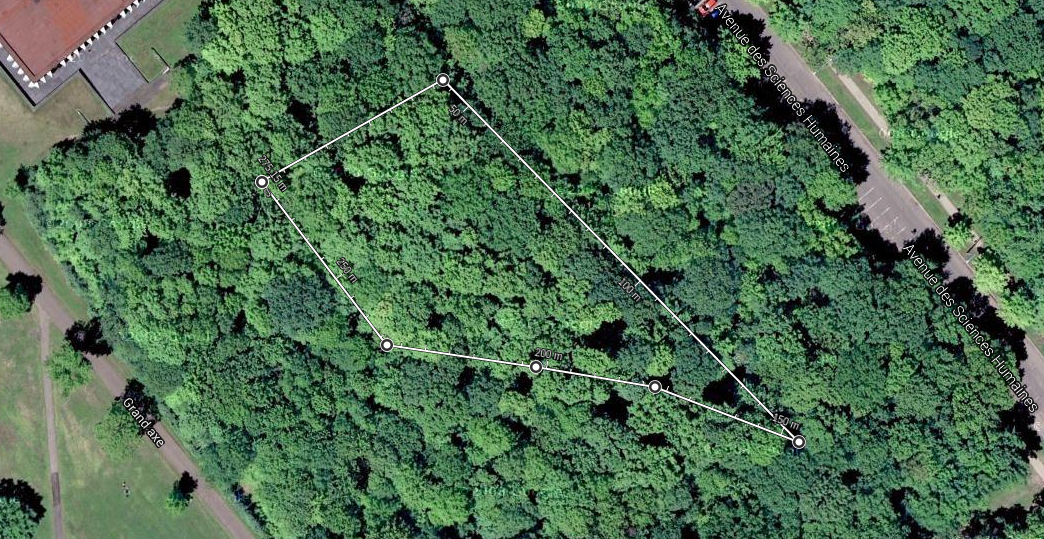
\includegraphics[width=0.92\linewidth]{./figures/path2.png}
            \caption{Google Maps. (2015).}
        \end{center}
        %\begin{figure}[]
            %\centering
            %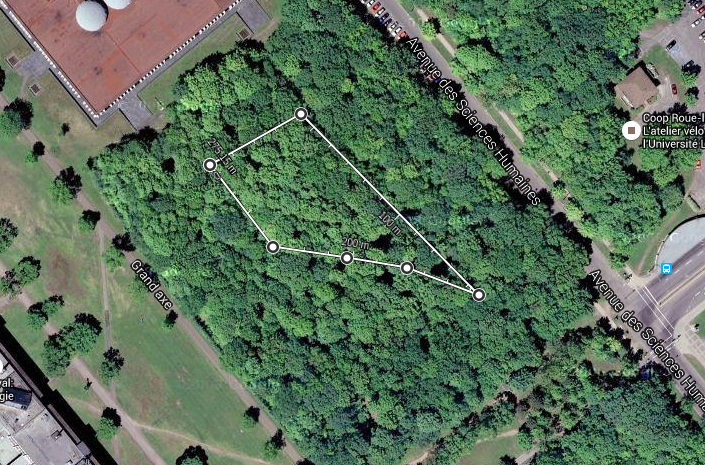
\includegraphics[width=0.8\linewidth]{./figures/path.png}
            %\caption{Approximative acquisition path (Google Maps. (2015))}
            %\label{fig:path}
        %\end{figure}
    }

    %----------------------------------------------------------------------------------------

\end{poster}

\end{document}
